
\documentclass[a4paper, 12pt]{article}
\usepackage[portuguese]{babel}
\usepackage[utf8]{inputenc}
\usepackage[T1]{fontenc}
\usepackage{indentfirst}
\usepackage{graphicx}
\usepackage{listings}
\usepackage{color}
\usepackage{fancyhdr}
\usepackage{xfrac}
\usepackage{float}
\usepackage{geometry}
\usepackage{caption}
\usepackage{blindtext}
\definecolor{mygreen}{RGB}{28,172,0}
\definecolor{mylilas}{RGB}{170,55,241}
\geometry{left=25mm, top=25mm, right=25mm, bottom=25mm}
\DeclareGraphicsExtensions{.pdf,.png,.jpg,.jpeg}
\captionsetup{labelformat=empty}

\lstset{language=Matlab,%
    %basicstyle=\color{red},
    breaklines=true,%
    morekeywords={matlab2tikz},
    keywordstyle=\color{blue},%
    morekeywords=[2]{1}, keywordstyle=[2]{\color{black}},
    identifierstyle=\color{black},%
    stringstyle=\color{mylilas},
    commentstyle=\color{mygreen},%
    showstringspaces=false,%without this there will be a symbol in the places where there is a space
    numbers=left,%
    numberstyle={\tiny \color{black}},% size of the numbers
    numbersep=9pt, % this defines how far the numbers are from the text
    emph=[1]{for,end,break},emphstyle=[1]\color{red}, %some words to emphasise
    %emph=[2]{word1,word2}, emphstyle=[2]{style},
}

\begin{document}
	\begin{titlepage}

		\newcommand{\HRule}{\rule{\linewidth}{0.5mm}}
		\centering
		\textsc{\LARGE Universidade de Brasília}\\[0.5cm]
		
\includegraphics{logo.jpg}\\[0.5cm]
		\textsc{\Large Instituto de Ciências Exatas}\\[0.5cm]
		\textsc{\Large Departamento de Ciência da Computação}\\[0.5cm]
		\textsc{\Large Princípios de Visão Computacional - Turma ``A''}\\[0.5cm]
		\HRule \\[0.4cm]
		{ \huge \bfseries Projeto Demonstrativo 1}\\[0.2cm]
		\HRule \\[3.0cm]
		\begin{minipage}{0.4\textwidth}
			\begin{flushleft} \large
				\emph{Nome:}\\
				\emph{Khalil Carsten}\\
				\emph{Renato Nobre}\\
			\end{flushleft}
		\end{minipage}
		~
		\begin{minipage}{0.4\textwidth}
			\begin{flushright} \large
				\emph{Matrícula:}\\
				\textsc{15/0134495}\\
				\textsc{15/0146698}\\
			\end{flushright}
		\end{minipage}\\[6.0cm]
		\textsc{\large \centering 4 de Setembro de 2017}\\
	\end{titlepage}

	\section*{Introdução}

    Detecção de elementos em imagens é uma parte essencial de diversas aplicações de visão computacional. Imagens possuem diversos elementos de interesse que podem ser usados com o objetivo de detectar outros aspectos da imagem. Altura de objetos, altura, rotação e foco da câmera, e distancia entre objetos.

    O objetivo deste projeto foi achar a altura conhecida de um elemento na imagem para achar a altura de outros elementos. Para isso foi calculado pontos de fuga, retas de fuga, linha do horizonte, e matriz de rotações $R$ em cinco imagens diferentes. O processo detalhado será discutido abaixo.

    \section*{Desenvolvimento}
		\subsection*{Compilação e Implementação dos algoritmos}
        Como primeiro passo visitamos o site de David Stutz onde são disponibilizados todos os links para os algoritmos
        usados no projeto, além de um repositório no $Github$ com um compilado dos mesmos.
        Por vários problemas com as bibliotecas usadas, baixamos cada algoritmo de seus respectivos
        sites e os implementamos separadamente. \par

        Depois de vários problemas para processar os superpixels nas fotos não tivemos sucesso
        ao instalar o CRS. \par

        Nas seções abaixo será apresentado os resultados dos processamentos e o agrupamento das
        imagens das folhas de acordo com a ordem da imagem original.


    \section*{ERGC - Eikonal-based Region Growing Clustering}
    Nesta seção serão mostrados os resultados do algoritmo ERGC no qual utiliza
    equação Eikonal e suas soluções para gerar os os cluster de pixels de acordo
    com [3] página 2.

		\begin{figure}[H]
			\centering
			\includegraphics[width=1\linewidth]{ERGC_final.png}
			\caption{Superpixel - ERGC}
		\end{figure}



    \section*{ERS - Entropy Rate Superpixel Segmentation}
    Nesta seção serão mostrados os resultados do algoritmo ERS onde este utiliza uma taxa
     de entropia em um caminho aleatório de um grafo e um fator de balaceamento do mesmo.
     Em cima disso os segmentos são formados em cima de uma ordenação topológica que maximixa
     uma função objetivo.

		\begin{figure}[H]
			\centering
			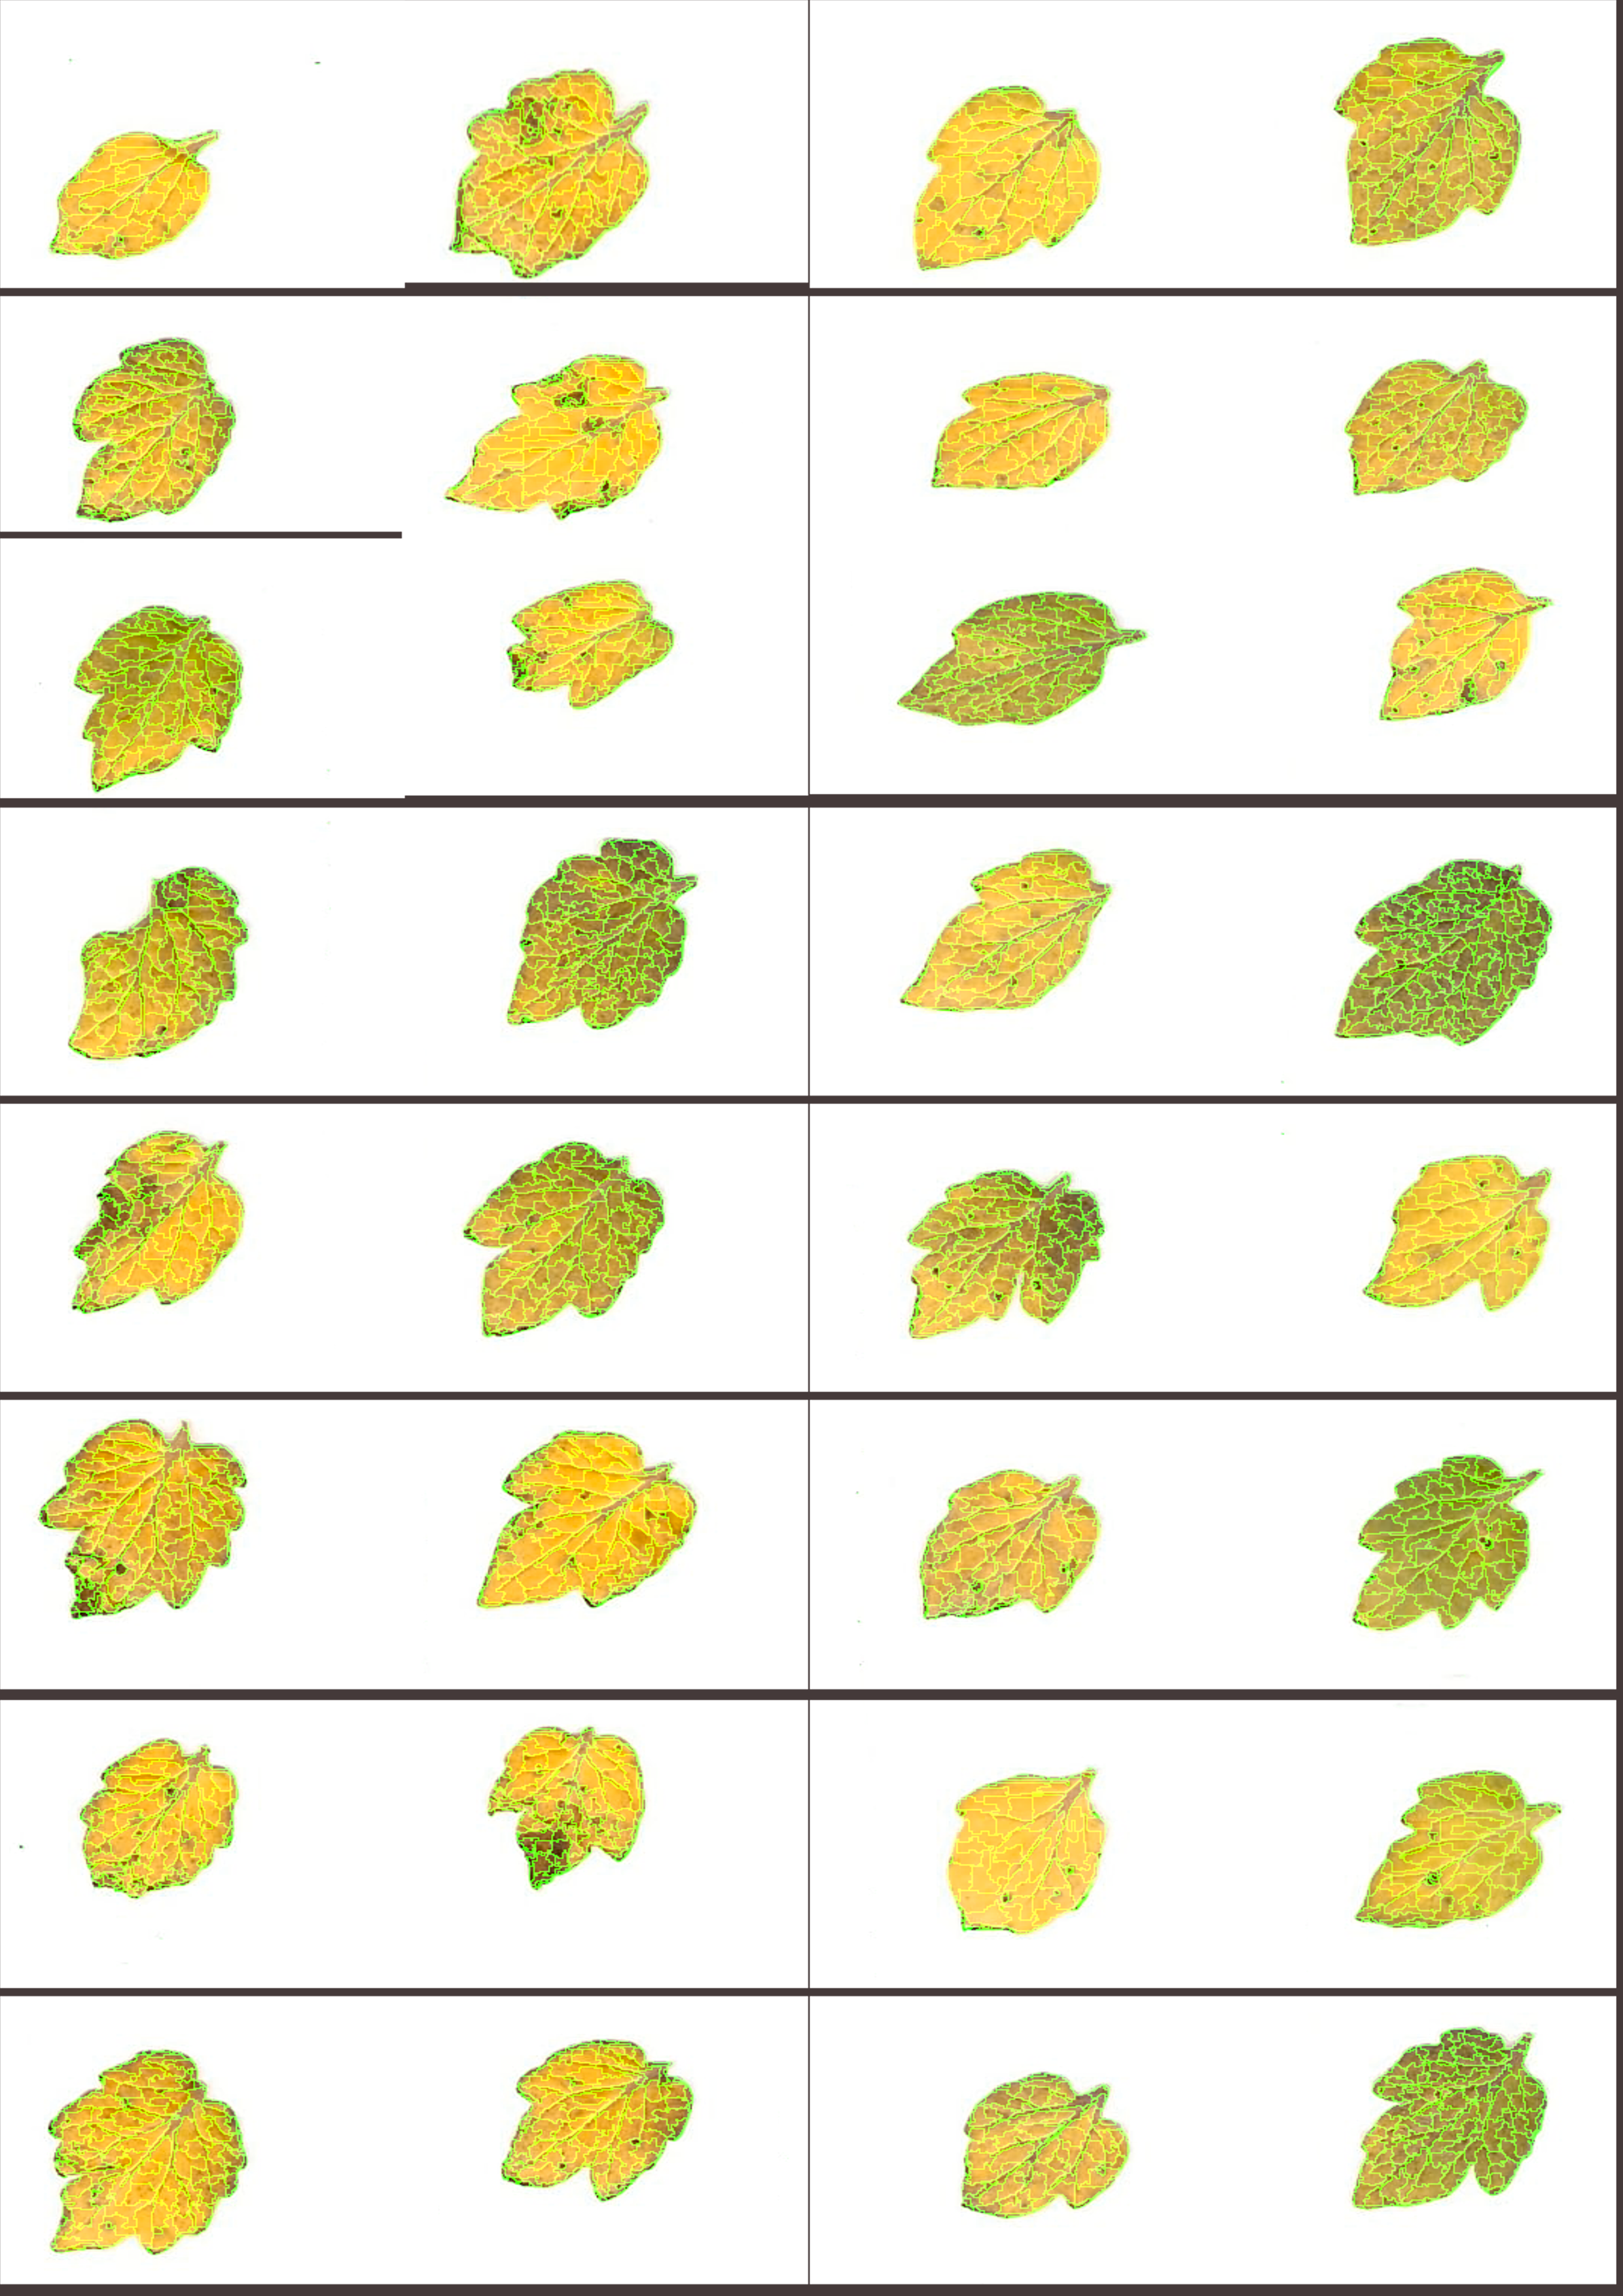
\includegraphics[width=1\linewidth]{ERS_final.png}
			\caption{Superpixel - ERS}
		\end{figure}

    \section*{ETPS - Real-time coarse-to-fine topologically preserving segmentation}
    Nesta seção serão mostrados os resultados do algoritmo ETPS onde este propõe uma otimização
    que diminui o número de interaçãoes. Baseado-se em algoritmos de SEEDS este utiliza métodos
    $coarse-to-fine$ para tal fim.

		\begin{figure}[H]
			\centering
			\includegraphics[width=1\linewidth]{ETPS_final.png}
			\caption{Superpixel - ETPS}
		\end{figure}

    \section*{SEEDS - Superpixels Extracted via Energy-Driven Sampling}
		\begin{figure}[H]
			\centering
			\includegraphics[width=1\linewidth]{SEED_final.png}
			\caption{Superpixel - SEEDS}
		\end{figure}

		\begin{figure}[H]
			\centering
			\includegraphics[width=1\linewidth]{SLIC_final.png}
			\caption{Superpixel - SLIC}
		\end{figure}

    \section*{Conclusão}
        O projeto realizado foi então validado comparando com a altura original das pessoas nas fotos a margem de erro é de aproximadamente 3 centímetros. A primeira pessoa que aparece nas duas primeiras imagens possui uma altura de $1.64$ metros, já a média da sua altura usando a altura encontrada nas as fotos foi de $1.61$ . Para a segunda pessoa, a média é de $1.72$, comparado com a altura real de $1.75$ metros.

        No entanto, o projeto apresenta certas dificuldades e limitações. Uma das principais dificuldades é em relação à disposição das fotos, que dependendo da maneira em que foi tirada pode se tornar impossível realizar os devidos cálculos. Outro ponto importante é que grande parte do projeto foi feito manualmente em vez de utilizar linhas de código para resolver o problema. Alguns passos podem ser automatizados, tais como, achar as linhas de fuga, o ponto de fuga, e detectar as pessoas nas imagens.

	\begin{thebibliography}{9}

        \bibitem{book1}
        Szeliski, Richard. ``Computer vision: algorithms and applications.'' Springer Science \& Business Media, 2010.

        \bibitem{slides}
        Slides de Aula

        \bibitem{book2}
        Pierre Buyssens, Isabelle Gardin, Su Ruan.``Eikonal based region growing for superpixels generation: Application to semi-supervised real time organ segmentation in CT images.'', 2015



    \end{thebibliography}



\end{document}
